\begin{frame}{Overview of Rational Proofs [AM12]}
\begin{itemize}[<+- | alert@+>]
	\item A variant of interactive proofs where the verifier pays the prover at the end;
	\item \textbf{Soundness:}
	\begin{itemize}
		\item ``A cheating worker gains less than an honest one''
	\end{itemize}
%	\item Other desiderata:
%	\begin{itemize}
%		\item Reward should be higher than cost (\textit{individually rational})
%		\item Ensuring ``significant'' losses for cheaters;
%		\item Ensuring ``compact'' budget for delegators.
%	\end{itemize}
\end{itemize}
\onslide<1->
\begin{figure}
	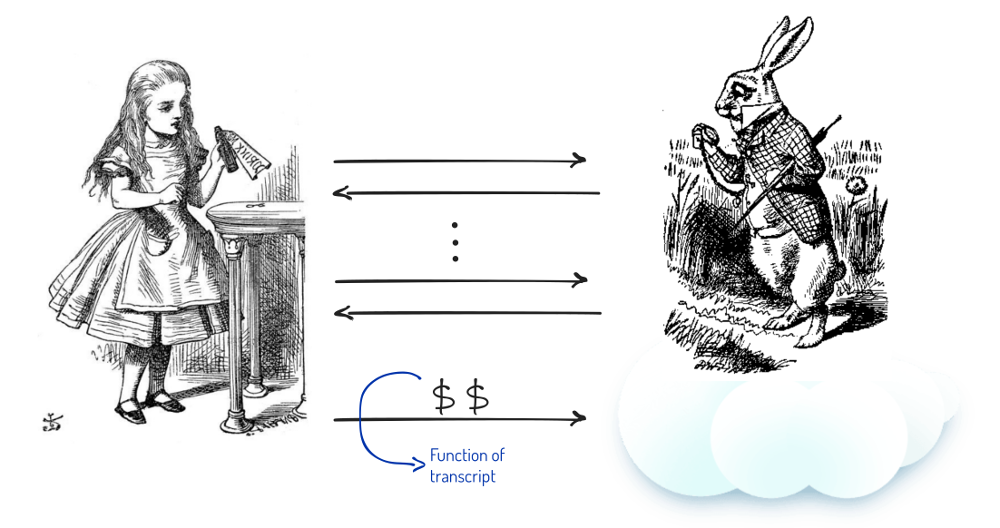
\includegraphics[scale=0.23]{pics/interaction.png}
\end{figure}
% Recall interactive proofs
% Recall our goal
\end{frame}


\begin{frame}{Rational Proofs: Definition [AM12]}
		\begin{framed}
			Let $f$ be a function and $(P,V)$ be a pair of algorithms. $(P,V)$ is a rational proof for $f$ if both:
			\onslide<+->
			\begin{enumerate}[<+- | alert@+>]
				\item \emph{("The honest prover always replies correctly")} 
				$$ \forall x\  \Pr[output(P,V)(x) = f(x) ] = 1$$
				\item \emph{("Any other prover will earn less than the honest one")}
				$$ \forall \disP \ \forall x \  \expRewProtHon - \expRewProtDis \geq \delta_{\disP}(x)  $$
				for some reward function $\rew$ and gap $\delta_{\disP}(x) \geq 0$
			\end{enumerate}
		\end{framed}
		
		%\pause
		%\vspace{0.5cm}
		%\center{\large{\textbf{What does $\rew$ look like?}}}
\end{frame}